\documentclass[5p,authoryear]{elsarticle}
\makeatletter 
\def\ps@pprintTitle{%
 \let\@oddhead\@empty
 \let\@evenhead\@empty
 \let\@evenfoot\@oddfoot} % Supprimer le bas de page ELSEVIER
\makeatother
\usepackage[utf8]{inputenc} % En unicode
\usepackage[T1]{fontenc}
\usepackage[english]{babel}
\usepackage[babel=true]{csquotes} % permet de faire \enquote{a} (« a »)
\usepackage{amsmath} % pour certains signes mathématiques
\usepackage{amsthm} % Pour \begin{gather}
\usepackage{booktabs} % pour \toprule (un style de tableau)
\usepackage{multirow} % Pour colonnes multiples des tableaux
\usepackage{amssymb} % Pour \leqslant (<=, >=)
\usepackage{float}
\usepackage{hyperref} % 
\usepackage[english]{cleveref} 

% adding Code Blocking
\usepackage{listings}
\usepackage{color}

\definecolor{dkgreen}{rgb}{0,0.6,0}
\definecolor{gray}{rgb}{0.5,0.5,0.5}
\definecolor{mauve}{rgb}{0.58,0,0.82}

\lstset{frame=tb,
  language=Java,
  aboveskip=3mm,
  belowskip=3mm,
  showstringspaces=false,
  columns=flexible,
  basicstyle={\small\ttfamily},
  numbers=none,
  numberstyle=\tiny\color{gray},
  keywordstyle=\color{blue},
  commentstyle=\color{dkgreen},
  stringstyle=\color{mauve},
  breaklines=true,
  breakatwhitespace=true,
  tabsize=3
}




%\bibliographystyle{elsarticle-num}
\bibliographystyle{elsarticle-harv}

\usepackage{fancyhdr}
\pagestyle{fancy}
\lhead{MSDS 453 - SEC 56}
\rhead{Lee, J.}

\begin{document}

\begin{frontmatter}

\title{Document Classification Model: \\NBA News Articles}
\author{Jason Lee}
\address{Northwestern University, SPS \\Natural Language Processing \\2020SP MSDS 453-56}


\begin{abstract}
Information is power in the sports betting industry. 
When team news hits the web, betting syndicates need to be able to react with speed before market prices adjust.
As web scrapers scour the internet collecting NBA news articles, a document classification model is needed to filter between the relevant information and irrelevant information.
The goal of this project is to determine the optimal vectorization and training process needed to build a high performing document classification model. 
A factorial experiment will be conducted with varying vector lengths and three key vectorization methodologies: 1) Analyst Judegment 2) TF-IDF 3) Doc2Vec Embedding. 
\end{abstract}


\begin{keyword}
Natural Language Processing (NLP) \sep Document Classification \sep NBA \sep Sports Betting \sep Python 
\end{keyword}

\end{frontmatter}


\section{Introduction}\label{introduction}

For professional sports bettors, determining what information is relevant as they are flooded with hundreds of news articles and "breaking news" alerts covering numerous leagues across all different types of sports is crucial for long term success. 
As focused web crawlers scrape the internet capturing up to the minute news about each team, there needs to be an automated process to filter out the irrelevant articles. 
This is exactly what a document classification model can do. 

A document classification model will be able to save a professional sports bettor countless hours by eliminating the manual effort needed to read the various news articles on each team and decide if it is useful.  
Building off of the corpus created by the focused web crawlers in the previous project, this project will center around the steps needed to create a finely tuned document classification model \citep{project1}. 

The predictive algorithm will be able to determine if a news article collected by the Spiders is relevant for the sports bettor or not. 
This automated filtering process, coupled with the focused web crawlers, will allow any sports bettor the ability to digest the right information in a timely manner. 

However, the process of building a document classification model is nuanced with success being dependent on the training corpus, vectorization methodology, vector length, algorithm selection, and number of predicted classes. 
A central component of this project will be to determine the optimal vector length and vectorization methodology to feed into the document classification model. 

Document vectorization is the operation used to convert a document of words into a representative, or meaningful, vector of numbers.
This is a required step to enable machine learning algorithms the capability to perform mathematical calculations when training classification models. 
The length of these document vectors can be adjusted with varying degrees of success to the model's outputs.

A factorial experiment will be conducted with three different methodologies to the vectorization of the NBA news article corpus as the first factor and the length of the vectors as the second factor. 

The three document vectorization approaches are as follows: 

\begin{enumerate}
 \item Analyst Judgment
 \item TF-IDF
 \item Neural Network Embedding
\end{enumerate} \\
 
The lengths of the document vectors will be 50, 150, and 300. 
Each vectorization approach with each vector length will be evaluated by fitting a random forest classifier and comparing the model's accuracy metrics, using the F1 score as the primary metric for optimization.  

\subsection{Analyst Judgment}

The Analyst Judgment methodology is a more "hands on" approach to document vectorization; it relies on the domain knowledge of the analyst. 
The analyst will need to determine which words should be the focal point in the vectorization process with two key criteria needing to be met, importance to the topic and prevalence throughout the corpus. 

\subsection{TF-IDF}

TF-IDF stands for Term Frequency-Inverse Document Frequency. 
The TF-IDF vertorization methodology is an algorithmic approach that involves using a weighted frequency count for words in the documents.
This equation is used to determine which words are important and prevalent throughout the entire corpus. 
Each word in the document will have their TF-IDF score computed and a subset of the highest valued words across the corpus will be used in a vector to represent each document.


\subsection{Neural Network Embedding}

The Neural Network Embedding methodology will utilize the deep learning Doc2Vec algorithm provided by the Gensim package in Python \citep{gensim}. 
This approach is an unsupervised approach where the neural network is trained in a similar fashion as the Word2Vec algorithm but with an additional input vector used as a proxy document identification number. 
By the end of the training process, each document identification vector weights will have updated in a way that becomes representative of the collection of words used in the given document \citep{doc2vec}. \\


The management problem this project addresses is the high cost of time and resources needed to manually filter through countless articles searching for information that could provide an edge for a professional sports bettor. 
Another issue addressed here is the speed to executing on this information. 
The sports bettor will need to react to important information before the markets have time to adjust. 
Automating this entire process with a document classification model will increase the return on investment for a professional sports bettors.

This natural language processing (NLP) project will also be a precursor for another NLP project focused on topic modeling using multivariate methods with unsupervised clustering algorithms, as well as multidimensional scaling. 
The output matrices from the three document vectorization approaches will be repurposed for the topic modeling algorithms.
A.I. Sports is the financial sponsor for this project and the classification models built herein will be implemented through their company to server their professional sports betting clientele \citep{aisports}. 

The following are the primary goals of this project:
\begin{enumerate}
 \item Create a calibrated document classification model.
 \item Determine which vectorization methodology produces the optimal results for this particular classification problem.
 \item Produce document vectors that will be used in future projects.
 \item Generate a reproducible Python workflow to easily share with colleagues. 
\end{enumerate} \\


\section{Literature Review}\label{lit_rev}

Document classification models are powerful natural language processing (NLP) algorithms that enable automated sorting and filtering systems to function independently of human intervention. Document classification models are designed to digest an entire document and return a predicted class \citep{chollet}. There are several data pre-processing steps and transformations that need to take place before a model can be trained. 

\subsection{Term Frequency-Inverse Document Frequency}\label{tf}

The Term Frequency-Inverse Document Frequency (TF-IDF) algorithm is a relatively simple but powerful approach to document vectorization and classification modeling. 

The actual equation consists of two components multiplied together as shown in Equation \ref{eq:1}, where \textit{t} is the given term. 
The first component is the term's frequency in the document (TF) and the second component is the term's inverse document frequency (IDF). 
\begin{equation}
    TFIDF(t) = TF(t) * IDF(t)\label{eq:1}
\end{equation}

Term Frequency (TF) is a normalized count metric for a given term. It is calculated by counting the number of times a given term is used in a document divided by the total number of terms in the document as shown in Equation \ref{eq:TF}, where \textit{t} is the given term and \textit{N} is the total number of terms in the document \citep{mining}.

\begin{equation}
    TF(t) = \frac{Freq(t)}{N}\label{eq:TF}
\end{equation}

Inverse Document Frequency (IDF) is calculated by taking the logarithm of total number of documents divided by the number of documents with the given term in it as shown in Equation \ref{eq:IDF}, where \textit{D} is the total number of documents in the corpus and \textit{D(t)} is the number of documents that contain the given \textit{t} term \citep{mining}. 
\begin{equation}
    IDF(t) = \log{\frac{D}{D(t)}}\label{eq:IDF}
\end{equation}

\begin{equation}
    TFIDF(t) = \frac{Freq(t)}{N} * \log{\frac{D}{D(t)}}\label{eq:TFIDF}
\end{equation}



\subsection{Neural Network Embedding}\label{Doc2Vec}

Conceptually, a neural network embedding algorithm places word, or term, vectors into a geometric space where the Euclidean distance between words, or terms, creates context and meaning \citep{chollet}. 
Once the terms are placed into a geometric space, mathematical equations involving words can be solved. 
For example, Equation \ref{eq:jazz} can be solved correctly with a properly trained neural network embedding model.
\begin{equation}
Utah\ Jazz - Utah + Miami = Miami\ Heat \label{eq:jazz}
\end{equation}

This may be a simple equation for an NBA fan to solve, but understanding the words’ relationship in this way for computers was a groundbreaking advancement. 
When working with documents, a popular neural network embedding solution is the Doc2Vec algorithm. 

To understand the intricacies of the Doc2Vec algorithm, there needs to be an understanding of the Word2Vec algorithm. 
The Word2Vec algorithm, created by Thomas Mikolov at Google, is a two-layer neural network that utilizes the bag of words and skip-gram architectures in parallel \citep{google}.


\subsubsection{Continuous Bag of Words (CBOW)}\label{Doc2Vec}

A Continuous Bag of Words network uses the nearby words to predict the target word \citep{lane}.
Figure \ref{cbow} displays that framework to show how this algorithm works \citep{word2vec}. 
The target word is in the middle having the two previous words and two proceeding words as the inputs.

\begin{figure}[!h] 
    \centering
	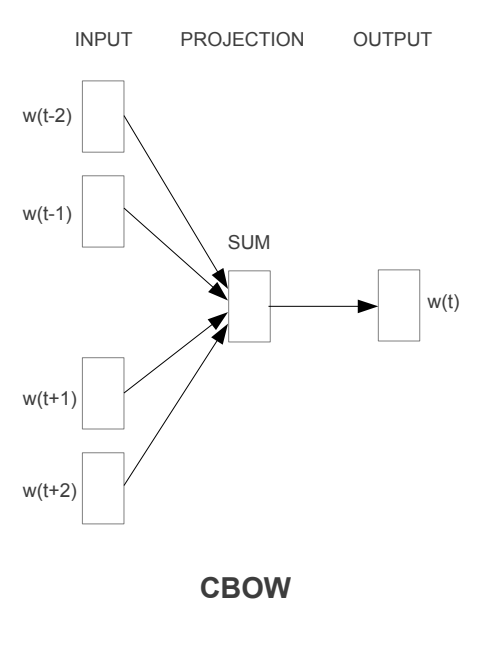
\includegraphics[width=2in]{figures/cbow.png}
	\caption[]{Framework of the Continuous Bag of Words model showing the inputs and output of a training sample.} 
	\label{cbow} 
\end{figure}



This window of five words slides over one word to create the next training sample.
Figure \ref{cbow_window} provides a diagram showing how this works. 
The red word is the target word and the other four words are the inputs.
The sliding window passes over the entire corpus creating a highly tuned model, especially with frequently used words \citep{lane}.

\begin{figure}[!h] 
    \centering
	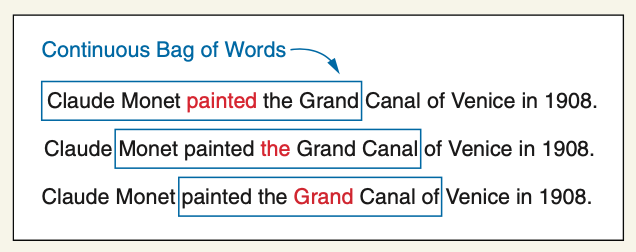
\includegraphics[width=2.8in]{figures/cbow_window.png}
	\caption[]{Sliding window of 5 words in the Continuous Bag of Words model.} 
	\label{cbow_window} 
\end{figure}


\subsubsection{Skip Gram}\label{skip}


The Skip Gram algorithm is the reverse process as the continuous Bag of Words model \citep{word2vec}. 
The input here is the given word and the goal is to predict the surrounding words as shown in Figure \ref{skip}.
The Skip Gram approach tends to perform better than the Continuous Bag of Words model when working with smaller corpora but takes longer to train \citep{lane}.

\begin{figure}[!h] 
    \centering
	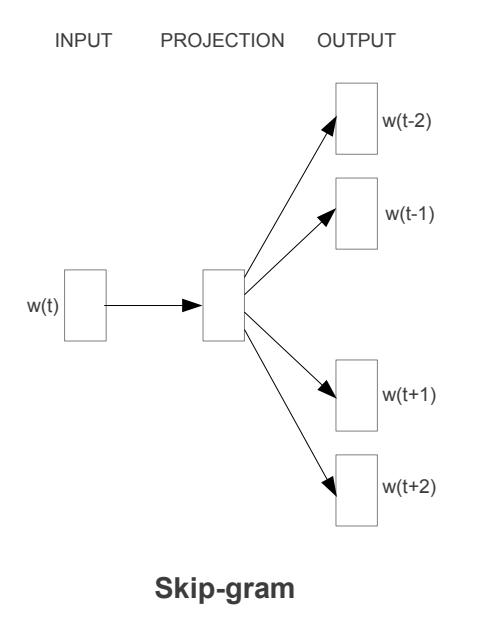
\includegraphics[width=2.2in]{figures/skip_gram.png}
	\caption[]{Framework of the Skip Gram model showing the input and outputs of a training sample.} 
	\label{skip} 
\end{figure}



\subsubsection{Doc2Vec}\label{Doc2Vec}

The Doc2Vec algorithm behaves similar to the previous algorithms, except it adds an additional input vector representing the document.\\



\begin{figure}[!h] 
    \centering
	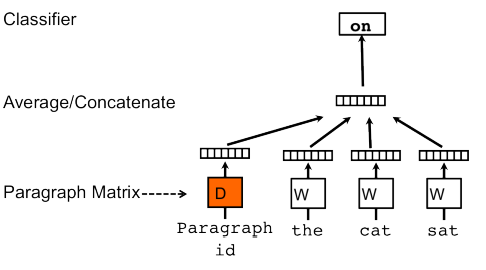
\includegraphics[width=3.4in]{figures/doc2vec_2.png}
	\caption[]{Doc2Vec training example} 
	\label{Doc2Vec2} 
\end{figure}


\begin{figure}[!h] 
    \centering
	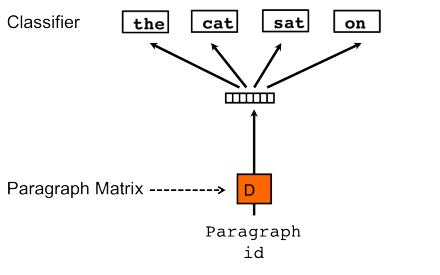
\includegraphics[width=3.4in]{figures/doc2vec_3.png}
	\caption[]{Doc2Vec prediction example} 
	\label{Doc2Vec3} 
\end{figure}


This document ID, or Paragraph ID in Figure \ref{Doc2Vec2}, is fed into the model and the weights in the document ID are updated along side the word vectors from its document \citep{doc2vec}. 
As the model converges during the training process, the document ID vector becomes Representative of the entire document in the new geometric space. 
Each document now has meaning and documents closer together in the geometric space have more in common than documents farther away. 
Figure \ref{Doc2Vec3} shows how the document ID can be used in a similar fashion as the Skip Gram model.

The draw back is that the neural network embedding algorithms are computationally expensive to train compared to other vectorization methods \citep{lane}. 

\section{Methodology}\label{meth}


The methodology implemented during this project is as follows. 


\subsection{Document Corpus}\label{corpus}

The corpus of documents that will be used in this project was collected by focused web crawlers, or Spiders. The Spiders were released onto each National Basketball Association (NBA) team's official website moving from page to page collecting six important pieces of information from every news article they came across.

\begin{enumerate}
 \item team  = The name of the NBA team
 \item url = The URL where the article is found
 \item tags = The topic tags for the article
 \item title = The title of the article
 \item date = The date the article was posted
 \item article = The complete news article
\end{enumerate} \\

The topics contained in this corpus are wide ranging. There are articles written about the team's humanitarian efforts, potential trades, pre-game/match-up analysis, injury updates, post-game analysis, deep dive player specific topics, player written articles, front office management news, team perception/fan sentiment, fan outreach, and miscellaneous articles.


\subsection{Dependent Variable}\label{dependent}

The document classification models built during this experiment will be designed to predict whether a news article provides relevant information for a sports bettor or not. The dependent variable is a binary flag. 

$$1 = Relevant$$
$$0 = Irrelevant$$

Topics that are included in the positive class include potential trades, pre-game/match-up analysis, injury updates, post-game analysis, and team perception/fan sentiment. Everything else will be contained in the Irrelevant class.


\subsection{Pre-Processing Corpus}\label{dependent}

The corpus will undergo extensive pre-processing before it will be able to be used in the experiment. The news articles are contain the raw text that was scraped from the websites creating 

After the corpus was cleaned there were 214,655 tokens, with the unique count at 14,022 tokens. This will be the vocab size (V) in the experiment. Figure \ref{word freq} shows the top ten most common words in the corpus.

\begin{figure}[!h] 
    \centering
	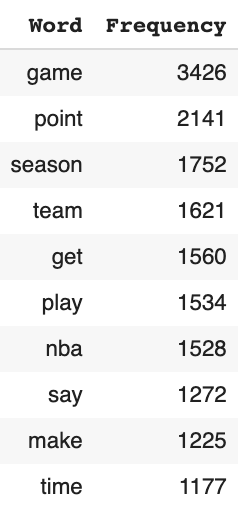
\includegraphics[width=1.4in]{figures/top_10_words.png}
	\caption[]{Top 10 words in the NBA news corpus} 
	\label{word freq} 
\end{figure}




\subsection{Factorial Experiment}\label{dependent}

In order to determine an optimal strategy for the vectorization of this corpus, a factorial experiment will be conducted. The experiment will consist of two factors with three levels each. The first factor will be the vectorization approach with the three levels as Analyst Judgment, TF-IDF, and Neural Network Embedding. The second factor will be the length of the vectors representing each document. The levels for the vector lengths are 50, 150, and 300.

There will be nine total document classification models built. The factorial experiment will hold all other parameters consistent allowing a clear interpretation of the interaction between the factors and the dependent variable. The nine classifiers will all be trained on the same random sample of documents, 70\% of the total corpus. These classifiers will then be judged on their effectiveness predicting the classes of the 30\% out of sample documents remaining.




\section{Computational Experiment}

The entire Python code for this project's factorial experiment will be attached to this paper, or can be reproduced by cloning the project's \href{https://colab.research.google.com/drive/10cnss2COB_KDHCvOy5tJGO7C56wtKYyw}{Google Colaboratory notebook} at this url:\\

\href{https://colab.research.google.com/drive/10cnss2COB_KDHCvOy5tJGO7C56wtKYyw}{Google Colab Link}\\ 

This script will begin by uploading and cleaning the NBA news article corpus followed by the experimentation with results. 
The experimentation portion of the Python code is an adapted version of the text classification example on the twenty newsgroup dataset \citep{sample-code}. 
There is an additional section in the Python script providing various data visualisations of the corpus.


\subsection{Analyst Judgment}\label{judge}



The Analyst Judgment methodology to vectorizing documents involves using the word statistics from the corpus. 
To easily generate the word statistics for this project, the CountVectorizer function from the SKLearn package in Python was used \citep{countVec}.
This function tokenizes the terms in the document and proceeds to count the number of times each token was used.

Using the domain knowledge of the analyst, a judgment was made to include bi-grams in these counts because of the importance gained by including groupings of words that are common in a sporting context. 
For example, "shot" is one of the most common words in the corpus and alone doesn't provide much value. 
However, when using bi-grams, a "missed shot", "made shot", "bad shot", and "good shot" are frequent terms in the relevant class and "flu shot", "action shot", "hot shot", "trick shot", and "snap shot" are more likely to be found in the irrelevant documents. "Shot" on its own appears more often in the relevant class but there will not be as much discrimination between the classes as using a bi-gram with "shot".

Another example is the word "Free". There is not much discrimination between between the classes on its own but when a bi-gram is used there is informative data. A "Free Throw" occurs during a game, making it relevant, but a "Free Car" is a promotional ad that is irrelevant. 

The CountVectorizer function was called three times to return a vector length of 50, 150, and 300. 
The returned vectors contain the number of times each term appeared in the document for the top 50, 150, and 300 terms respectively. 
Often this method produces sparse vectors but limiting the number of features will mitigate this issue \citep{LeeCount}.

The CountVectorizer only used the vocabulary in the training dataset to avoid any leakage or bias in the experiement. 
If there are terms in the test dataset that were not included in the training dataset then the function will simply disregard them. 


\subsection{TF-IDF}\label{tfidf}

The Term Frequency-Inverse Document Frequency (TF-IDF) approach is similar to the analyst judgment in that they both use word statistics from the corpus. 
In fact, the CountVectorizer function followed by the TfidfTransformer will produce the same results as the TF-IDF equation. 

For the experiment, the TfidfVectorizer function from the SKLearn package will be used to calculate the TF-IDF values for each term in the corpus \citep{tfidf}. 
Bi-grams will be used in this approach to remain consistent with the Analyst Judgment approach.


\subsection{Neural Network Embedding (Doc2Vec)}\label{exploration}

The final methodology to vectorizing the documents in the corpus is training a neural network embedding algorithm using Doc2Vec provided by way of the Gensim package in Python \citep{gensim}. 

This methodology was produced substantially longer transformation and training times than the other approaches. The other approaches took roughly 0.7 of a second, while the Doc2Vec approach took 40+ seconds. That is 57 times longer.

\section{Results}

Each of the nine document classification models in this experiment were fit using a Random Forest algorithm.
The out of sample test dataset with 231 documents was used as a measuring stick for each vectorization methodology and vector length. 
The F1 Score, harmonic mean between the precision and recall metrics, is the primary indicator used to evaluate the usefulness of each document classification model. 

The F1 Score results for the factorial experiment are contained in Table \ref{table_eval}.


\begin{center}
\begin{table}[!htb] 
  \centering 
  %\caption{\textbf{F1 Score - Harmonic Mean of Precision and Recall}}
  \begin{tabular}{r|c c c} %{@{\small}llll@{}} 
    \toprule % utilise booktabs
    \footnotesize \textbf{Vector} & \multicolumn{3}{c}{\textbf{Methodology}} \\
    {\footnotesize \textbf{Length} & {\footnotesize \textbf{Analyst}} &  {\footnotesize \textbf{TF-IDF}} & {\footnotesize \textbf{Embedding}}} \\
    \midrule
    50 & 0.835 & 0.838 & 0.821 \\
    150 & 0.844 & 0.822 & 0.767 \\
    300 & 0.820 & 0.818 & 0.743 \\
    \bottomrule
\end{tabular} \caption{F1 Score - Harmonic Mean of Precision and Recall} 
\label{table_eval}
\end{table}
\end{center}

The optimal document vectorization methodology for this particular document classification model is the Analyst Judgement. 
For every vector length, the Analyst Judgment approach reigned supreme. 
The Analyst Judgment with a vector length of 150 was the best performing classifier. 


\section{Discussion and Conclusions}

The results from this experiment are not that surprising. 
The classification problem is a simple binary indicator in a domain where the relevant articles will all contain very similar words. 
The irrelevant class contains a wider variety of words and topics. 
The Analyst Judgment document vectorization methodology is able to correctly prioritize key words to attain strong discrimination between classes.

In conclusion, this project was able to accomplish each of the four goals originally laid out. 
A well calibrated document classification model was built that will be used by A.I. Sports when sporting events return from the COVID-19 hiatus. 
The first approach, Analyst Judgement, proved to be the most effective document vectorization methodology.
The document vectors have been saved for future projects.
And finally, a fully reproducible Python script was programmed that can be easily shared with others. 

\clearpage

\bibliography{bibliographie.bib}

\bibliographystyle{newapa}

\end{document}